% !BIB program = biber

\documentclass[12pt,a4 paper,title page]{article}
\usepackage[utf8]{inputenc}
\usepackage{microtype}
\usepackage[british]{datetime2} % For urldate formatting
\usepackage{natbib}
\usepackage{graphicx}
\usepackage{float}
\usepackage{textcomp}
\usepackage{xcolor}
\usepackage{soul,color}
\usepackage{amsthm}
\usepackage{bm}
\usepackage{algorithm}
\usepackage{algorithmic}
\usepackage{amsmath,amssymb,amsfonts}
\usepackage[nottoc,notlot,notlof]{tocbibind}

\theoremstyle{definition}
\newtheorem{definition}{Definition}[section]
% \renewcommand{\algorithmicrequire}{ \textbf{Input:}} %Use Input in the format of Algorithm  
% \renewcommand{\algorithmicensure}{ \textbf{Output:}} %UseOutput in the format of Algorithm 

\usepackage[colorlinks = true,
            linkcolor = teal,
            urlcolor  = teal,
            citecolor = blue,
            anchorcolor = blue]{hyperref}
\usepackage{wrapfig}



\bibliographystyle{uts} % Import Harvard UTS style
\setcitestyle{aysep={}} % Remove comma separation between author and year for in-text citations

\title{Research Proposal: Adaptive Recommender System with Knowledge Graph}
\author{\large\textbf{Di Zhang}, \\
\textbf{supervisor: Professor Guanquan Zhang}, \\
\textbf{co-supervisor: Professor Jie Lu, Phd. Qian Zhang}, \\
\textbf{Student number: 31292711}}

\date{\Large{\textbf{Aug 2020}}}

\begin{document}
\sloppy
\maketitle

\tableofcontents
\newpage

%!TEX root = main.tex

\section*{Abstracts}
T.B.D.

\subsection*{Keywords} 
Recommender system, Heterogeneous Information Network, Knowledge Graph, Transfer Learning, Feature Representation Learning

\section{Introduction and background}
Recommender System (RS) is an indispensable technology, it evolves around our everyday life on multiple fronts. RS help us to find personalized interests from information overloads \citep{Lu2015}. It can act as a decision assisting agents to simplify or accelerate decision making process. Further more, as we experiencing the exponential growth of data content, RS keeps us updated on new emerging information.
Over the years, we see RS being adopted across different industries. At the same time, we noticed that, bringing a recommender systems into real-world application often faces many different sorts of challenges. 

Recommender systems exists long before computer was invented. Catalogs can be considered a one of the most primitive content-based recommender systems. In 2006, 100 million datasets were released by Netflix \citep{Bennett2007} The action expedited the research on Collaborative Filtering (CF). Over decades, Matrix Factorization based approach is still at the forefront of Recommender systems Field. Many new approaches and extensions had been evolved based on Collaborative Filtering to tackle its computation challenges and data sparsity problems. 

Transfer Learning \citep{Pan2010} in Cross Domain recommender system is another promising area which allowing recommendation possible in when initial user interaction data is scarce in target domains. \citet{Elkahky2015} experimented this approach on multiple Microsoft products, and concluded multi domain recommender system significantly outperforms single domain recommender systems. 


Meanwhile, building recommender system requires systematic approach, beyond algorithm and statistical analytics. Being overwhelmingly popular, CF's success is not only due to its effectiveness, but also thanks to its simplicity and low barrier of entry \citep{Amatriain2016}, despite of having known issue with data sparsity and cold start problems. Based on research observation, the challenges of setting up a successful real-world recommender system mainly comes down to 3 parts:  

\begin{itemize}
\item Algorithm. Setting up an effective recommender system is different for every business and every problem. A algorithm in recommender system is very hard to kept generic. Thus, transferability and reusability is low.

\item Data Adaptation. In the real-world scenario, information in flow as data streams. Features changes as time go by, along with recommendation objective. We often see diminishing performance from a developed recommender system over time. The ability to adapt data and making use of new emerging information remain challenging in recommendation field.

\item Feature Representation. Researcher and developers normally facing enormous yet complex datasets, in which, only small percentage can be effectively utilized. A generic yet effective learning methodology is a key building block to overcome data sparsity and cold start problems for recommender systems.
\end{itemize}

Living in a world of information, the information objects or data points around us are mostly interconnected with each other as a Heterogenous Network. World wide web, biology networks, as well as traffic system, etc. can all be formed into an information network. In our research, we consider knowledge graph as heterogeneous information network having a lot of promising potential in developing generic recommendation framework for solving challenges above.

This study will focusing on leverage knowledge graph to improve early stages recommender systems prediction capability and accuracy. The rest of this report is organized as follows: 
First we go through research questions, objectives and expected outcomes in Section 2. Next, in section 3, we present an extensive literature review of the related work of this study. It will cover recent recommender systems, knowledge graph representation and transfer learning research results. Section 4 describes the significance and innovation of this research. Section 5 presents the methodology to conduct this research. Section 6 is about the ethics and risk consideration. Finally, Section 7 outlines the entire timeline of this research and reports on the research progress up-to-date.




\section{Research Question, Objectives, and Expected Outcome}

\subsection{Thesis statement and Questions}
By learning rich semantic information of knowledge graph can help in developing recommender systems, that is capable of maintaining effectiveness overtime with relative low maintenance cost. 

\subsubsection*{Question 1}
How to present users and items in a heterogeneous information graph for recommendation problems?

\subsubsection*{Question 2}
How to effectively transfer knowledge to assist recommendation among multiple domains with knowledge graph?

\subsubsection*{Question 3}
How to develop a dynamic recommendation system that is adaptive to data changes overtime?

\subsection{Objectives}
This research aim to achieve following objectives: 

\subsubsection*{Objective 1: To develop a graph based approach that can taking account of complex metadata for various recommendation problems.}

Taking Collaborative Filtering based recommendation systems for example, commonly the model only uses user-item interactions dataset in training. Fusing item or user explicit information as part of Collaborative Filtering training are often very challenging and can hits computation or memory bottlenecks easily. Similar challenges apply to content based recommendation systems as well, where importance across multiple features become difficult to balance during the feature engineering process.

In this study, By leveraging the heterogeneous network structure, user-item interactions, as well as users/items attributes, can be naturally fused in to single Multiple-Hub Network \citep{Shi2017} structure. Hence, a generic approach, that project users, items, and their related feature information into heterogeneous Information Network, can be developed for accommodating richer information in recommendation model training.

% \textbf{Success condition:} Load raw data set into a graph structure that can effective present the information required for recommendation problem accordingly 


\subsubsection*{Objective 2}
To develope a graph embedding based method that is capable of dealing data sparsity and cold start problem.

% For the heterogenous information graph, evaluate the similarity of objects is the fundamental in data mining. In recommender system, it faces ever growing and evolving dataset. Working against massive datasets, and complex data transformation are common obstacles for producing a high quality recommendation solution. Developing an computational efficient similarity measure that fits for recommender system's use case, is a key milestone to ensure my research success.

% \textbf{Success condition:} Evaluate current graph-based similarity measures to determine and develop a fitting similarity approach for recommender system, which is, capable of solving Top-K recommendation and effective in Cold Start problems. 


\subsubsection*{Objective 3}
To develop a graph based detection method to detect recommendation effectiveness and user-interest drift.

% The rich information contained within the same HIN may only useful for certain recommendation problems. Nodes and path would have different weights when optimization objective or time is different. Developing a semi-supervised mining method would help recommender system to find different weights on based on the inter relationship between nodes and meta-paths. Reducing complex features into lower dimensions would also helping reduce the computation complex \citep{Cai2018} as mentioned in Object 2, Further simplify implementation difficulties in recommender systems. 

% \textbf{Success condition:} An embedding approach that is not only performant but also computational effective for mining large scale HIN. 


\subsubsection*{Objective 4}
To develop a graph neural network based recommendation method that is adaptive to new emerging data points.

% Time factor is an important factor for making recommendations. Users past context could have direct impact of user current interest. \citet{Song2019} had shown that measurable improvement performance can be found in recommender system, when exploiting time information in the recommendation process. As a extension objective from Objective 2 and 3, including temporal dynamics and considering the transitive similarity between nodes and edges is another important factor in delivering quality results.

% \textbf{Success condition:} A graph-based framework that is capable learning feature changes over time. 

\subsubsection*{Objective 5}
To develop a transfer learning method based on Graph Neural Networks for cross domain recommendations.

% By putting research results from Objective 1,2,3 into a holistic framework, would enable us to develop a generic approach and making recommendation model adapting changes could significantly reduce the recommendation systems maintenance cost and keeping system performance over time. 
% Instead of focusing the recommendation research on static datasets. In this research, we are trying to solve the real-world recommendation problem in a dynamic angle.

% \textbf{Success condition:} A working recommender framework prototype using generic approach that is capable to  adapting to feature change and computational effective.  

\subsubsection*{Objective 6}
To develop a recommender system case study for validating the proposed approaches.

Following common datasets will be used for method verification: 

\begin{itemize}

\item MovieLens dataset (http://grouplens.org/datasets/movielens/) 

\item Netflix dataset (http://www.lifecrunch.biz/archives/207) 

\item DBLP Citation Networks (https://dblp.uni-trier.de)  

\end{itemize}

Case studies on real estate and tourism recommendation will be conducted to validate the user-interest drifts overtime, to show how graph-based approach adapts to the ever-evolving data changes. 


\section{Literature Review}
In this literature review, we will first cover a brief overview of classic single domain recommender systems. Then, we will dive deeper into existing knowledge graph based node representation studies, which explores the knowledge graph application for improving the recommendation model's adaptiveness and its effect on reducing cold start impact. Lastly, we will go through some existing cross-domain recommendation techniques and its recent development in association with the knowledge graph for feature enrichment and model adaptation.

\subsection{Recommender systems}
Recommender systems can be regarded as a algorithmic decision-making strategy, which contain a set of measure, analysis and prediction algorithms. It is capable of predicting users interests under large and complex information environment.

\bigskip
\subsubsection{Collaborative Filtering based recommender systems}
Collaborative filtering (CF) based recommender systems are one of the most widely used recommender systems. The key intuition of the model, that is similar users share similar interests in item preferences, and vice versa. CF can further divided into memory base CF, model based CF, and hybrid models.

Neighborhood-based top-N recommendations are typical example of memory-based CF. The core part in the memory-based approach is to find similarity through the nearest neighbor algorithm on users or items. Cosine similarity or Pearson correlation coefficient \citep{sarwar2001item} are commonly used for similarity measures. Rating is then aggregated based on similar users/items, lastly items are sorted according to the calculated scores as a ranked list for the target user. 

Matrix Factorization and data mining techniques are frequently used in model-based CF. There are many model-based CF algorithms. Bayesian networks, clustering models, just to name a few. The general approach is using machine learning pattern recognition ability to map complex pattern from large sparse data matrix into dense low-dimensional representation. Base on different recommendation objectives, different optimization strategy is applied. i.e. Mean squared deviation is commonly used for explicit rating estimation, while Bayesian personalized ranking (BPR) \citep{rendle2012bpr}, a pair-wise ranking optimization criterion, is widely used for implicit click-through prediction.   
Meanwhile, item2vec \citep{barkan2016item2vec} is a good example of data mining in recommendation applications. Inspired from word2vec \citep{mikolov2013distributed} Skip-Gram algorithm, item2vec treats each item as a corpus, then shuffles items order during the training process. In the end, items are embedded into a multi-dimensional vector space. So that, similarity between items can be easily measured by calculating the distance without supervision.  

There are two major problems with CF-based approach.  
One is, when user and item number grows exponentially, collaborative filtering is unable to scale up easily, which limits its ability in making recommendation on large datasets. Some dimensional reduction technique can help, in terms of reducing the matrix size. However, we could also fall into the risks of information loss, which leads to accuracy degradation. 
The other glaring problem for matrix factorization algorithm is data sparsity. Sparsity problem could happen when user interaction data only covers small percentage of the total item data set. The other common case is cold start, which is, when user or item newly enters into the system. Due to the lack of new item or new user interaction histories, this makes collaborative filtering unable to make meaningful predictions.  
Techniques such as singular value decomposition, latent semantic indexing is adopted to alleviate the sparsity problem. Those techniques try to improve the performance by filtering out unusable user-item representations and reducing dimensional space. However, such techniques could also have side effects, such as information loss. 

From implementation and real-world adaptation perspective, there are some simple yet practical ways of solving new user cold start problems without rely on Machine Learning or Data Ming. For example, Netflix gives user survey on users signing up process. Then the collected data is feed into its Recommender model to archive better user retention rate \citep{gomez2015netflix}. however in general CF-based model still faces complexity challenges, when it comes to feature engineering and maintenance cost. 


\bigskip
\subsubsection{Content based recommender systems}

Content-based recommendation methods are dependent on the individual user’s own historical records regardless of other users interaction. This making it different from the CF-based recommendation methods. 
As suggested by the name , content-based recommendation methods aim to recommend items based on contents that are matching to users previous interests \citep{shardanand1995social}. The content-based recommendation methods derive from information retrieval and focus on items with text information such as documents, or categorical attributes. For example, users who interested in job posts that requires ``python'' and ``machine learning'' is likely prefer to see more job listing that requires similar skills. 

There are 3 basic steps in content-based recommendation methods are: 
\begin{itemize}
    \item definition of important and discriminate item feature and attributes for item representation;
    \item determination of the principal common attributes as users preference profile based on individual users' historical interaction;
    \item matching users profile with items attributes, and recommendation generation base on matching scores.
\end{itemize}

Though content-based recommender system is more capable of handling cold start substitutions. The challenges of building such recommendation model are most related to the complexity of defining feature importance which leads to inability of adapting to data changes. The feature selection process is also heavily depended on experts domain knowledge. 

\subsection{Knowledge graph based recommender systems}
Known for its semantic properties, knowledge graph captures information and relationship between different types of data entities. Comparing with traditional column-based data structure, It is much more adaptive to constant data updates. 

Techniques such PathSim \citep{Sun2011PathSim} and HeteSim \citep{Shi2013HeteSim} provided a rich foundation for similarity measurements. Its results can be naturally borrowed into recommender systems. 
Embedding based approach, such as node2vec \citep{grover2016node2vec} further pushed graph based algorithmic framework for learning continuous feature representations. In node2vec, nodes is mapped to low-dimensional space of features that maximizes the likelihood of preserving network neighborhoods of nodes. Using a biased random walk procedure to explores diverse neighborhoods, node2vec can learn task-independent representations in complex networks. 
Entity2rec \citep{palumbo2017entity2rec} demonstrated that by using knowledge-graph, property-specific user-item relatedness, and global user-item relatedness, could significantly improve top-N recommendation performance

Graph neural network approach, such as, graph convolution network \citep{kipf2016semi} have shown promising results in node representation space. 
GraphSAGE \citep{hamilton2017inductive} proposed an inductive approach for generating node embeddings. Instead of requiring all nodes in the graph to be presented during training of the embeddings, GraphSAGE extend the generalization ability to unseen nodes. 
Graph attention network \citep{lee2018graph} is a good demonstration of attention-based learning techniques are applied in graph. Such feature learning ability makes a graph based data feature to be more versatile in facing data changes. 
Techniques, such as, user-guided embedding, can be invaluable for catering to optimise recommendation problem and effectively reduce the data noise problem by exploiting the signals residing in the data.

GNN research also intrigued applications in the recommendation domain. \citet{ying2018graph} shows promising signs of GNN being adopted in a large-scale deep recommendation engine. \citet{song2019session} propose a recommender system that model dynamic user behaviors and context-dependent social influence with a graph-attention neural network, which dynamically infers the influencer based on users’ current interests. Both of the research shown that GNN would be a promising approach for making the recommender systems more adaptive and capable of handling cold start problems.

\subsection{Cross-domain based recommender systems}
Recommender systems can be built from two or more different but related domains \citep{fernandez2012cross}.

User/item clustering and domain adaptation strategy are commonly used approaches for knowledge extraction between the source and target domain. Such as, Consistent Information Transfer (CIT) \citep{zhang2017cross}, where flexible mixture model is used to cluster the users and items separately \citep{si2003flexible}, then geodesic flow kernel is used as a domain adaptation strategy to align the user and item latent feature spaces \citep{gong2014learning}.

Kernel-induced Knowledge Transfer (KerKT) uses constraints on similarities between the entities in each domain as a bridge for knowledge transfer \citep{zhang2018cross}. It is important to maintain the intra-domain and inter-domain entity similarities, while measuring the similarities between entities in the same domain are easy, inter-domain entity similarities cannot be computed directly.
KerKT has a strong connection to a bipartite edge completion problem\citep{he2016birank}. We use connected nodes in the graph representations for both the source and target domains. The overlapping entity naturally act as ``bridge'' to couple the two domains.
As a result, The overlapping entities are mapped and measured in the same feature space for similarities, subsequently, the non-overlapping entities similarities can be then measured by diffusion kernel completion.

In recent years, many graph based transfer learning method had emerged. GANs \citep{goodfellow2014generative} base domain adaptation strategy are found in graph convolution methods \citep{dai2019network}. While \citet{xi2020graph} use graph factorization machine for cross-domain recommendations. It first projects nodes from both domains graph into a low dimension dense vector. Then its framework leverage message propagation and shared graph parameters to combine both domain specific and overlapped features for prediction task.

One reason to exploit cross-domain recommender systems is solving data insufficiency problem in single domain. As one domain may borrow relatively rich data insights from the other domain. While the available data in source domain can assist with the recommendation in a target domain with sparse data. 




\section{Future Significance}

\subsection{Practical Significance}
This research develops an adaptive recommendation framework based on cross-domain knowledge graphs, which improves recommender systems adaptiveness to new emerging information, even under constrained data conditions.

Data sparsity and quality issue are big barriers in a real-world recommender system production process, which often leads to poor prediction performance. The recommendation model are more prone to have cold start problems, due to the limited data during training. In this research, we illustrated a systematic framework to overcome above challenges. A holistic approach is introduced, that combines knowledge graph, representation learning, and knowledge transfer learning into a end-to-end schema. Consequently, the proposed approach reduces engineering effort and cost of building such a recommender system, allowing wider business adoptions.


\subsection{Theoretical Significance}
This research develops an adaptive recommendation framework that could greatly improves the recommendation performance under sparse data and cold start conditions.

Knowledge graph based representation and cross-domain transfer learning technique is combined as a unified framework to enrich and extract user item information for improved data density and richer node representation. 

Inside the heterogenous knowledge graph, user item metadata, as well as user-item interactions are natively preserved (connected) via nodes and edges within the graph structure. Its rich connections enables new incoming nodes to be incorporated into the graph organically. By leveraging message propagation and aggregation rules, even unseen user or item representation can be generated inductively for recommender system use. As a result, the research outcome would makes the recommendation model more adaptive to cold start problems.

% Research leverages graph based message propagation and aggregation ability

% Most of the recommender system research treats recommendation problem as a static snapshot. The consequences of such approach means the recommendation model's ability of adapting new data points are low. Data changes are rarely scoped as part of recommender system design, even though that is a key characterize of real-world datasets. 

% For this study, we are focusing on recommender systems design by leverage knowledge graph structure. We explore the entity representation property inside heterogeneous graph and its knowledge transferring ability under cross-domain settings to improve recommendation quality and model adaptiveness, especially, when initial datasets are sparse.




\section{Methodology}

\subsection{Task 1: propose a graph structure modeling methodology for recommender system}
It is challenging to develop effective data extraction and exploitation methods for Heterogeneous Information Network based recommender system.

\subsubsection*{Step 1: develop a generic graph structured data for recommendation problem}

Graph structure is being adopted in a wide range of applications. However, to our best of knowledge, none of them is taking a generic approach in forming the heterogeneous graph for recommender systems. HIN normally only optimized for a specific problem, and less adaptable to information evolution over time. 
Based on the nature of recommender system, we propose to accommodate not only user-item interaction, item features, and user profile information into the same heterogeneous information network. We also propose to further explore the semantic information by normalizing features on both item feature and user profile information into more atomic feature nodes. such practice would bring multiple benefits: 

\begin{itemize}
    
\item[1] Reduce data sparsity. By breaking up item features into more generic feature nodes would help increase the density of the network, and increase possible connectivity (mate-path) between nodes.

\item[2] With that, new in coming information would also transformed through the same decomposing process, hence making the graph structure adaptable to ever evolving changes.

\item[3] As the information graph cumulates auxiliary information in a holistic approach, suc structure also making problem context switch possible.

\end{itemize}

Of course, having a generic purpose HIN as training source introduce both complexity and noise. which we would discuss in Task 2 and Task 3.


\subsubsection*{Step 2: to develop transformation rule for the graph structure}

Recommendation test data sets are normally saved in csv format, which is quite different from the graph data structure we proposed above. Multi-Hub Network structure will be developed to transform the flat user-item data sets into a holistic feature-rich graph structure. Fig. \ref{fig:multihub}

\begin{figure*}[!t]
    \centering
    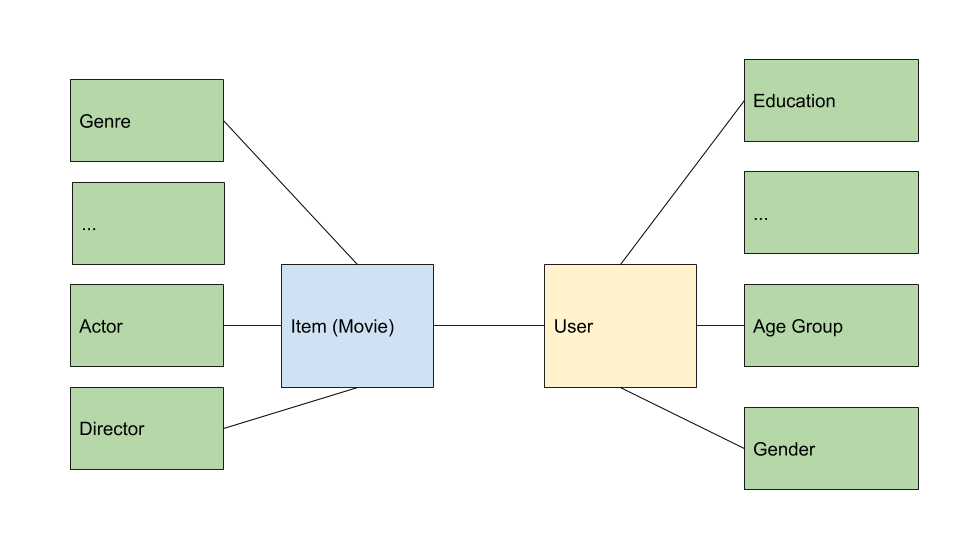
\includegraphics[width=0.8\textwidth]{figs/multi-hub.png}
    \caption{a multi-hub network structure based on Movielens data}\label{fig:multihub}
\end{figure*}


\subsection{Task 2: develop a comprehensive graph similarity measure}

Similarity measure the basis of many recommendation tasks, It evaluate the proximity among objects. Feature-based and link-based approaches are 2 main Similarity measures in HIN. 

The feature based approaches measure the similarity of objects based on their feature values, such as cosine similarity, Jaccard coefficient, and Euclidean distance. The link based approaches measure the similarity of objects based on their link structures in a graph. 

Similarity measure on HIN not only considers structure similarity of two objects but also takes the meta-path between two objects into account \citep{Shi2017}. \citet{Sun2011PathSim} propose PathSim that measure the semantics structure in meta-paths constituted by different-typed objects. The intuition for a single Meta-Path measure can be seen as: if source entity and target entity are exactly the same, then the round trip Meta-Paths $\mathcal{P}_1: A_1 \xrightarrow{r_1} A_2$ and 
$\mathcal{P}_1^{-1}: A_2 \xrightarrow{r_1^{-1}} A_1$ are always symmetric.

\theoremstyle{definition}
\begin{definition}[PathSim \cite{Sun2011PathSim}]\label{def:pathsim}
    Given a Meta-Path $\mathcal{P}$, PathSim between two entities $x$ and $y$ is:
    \begin{equation}
        sim(x,y)=\frac{2 \times \{|p_\text{x...y}:p_\text{y...x}| \in P\}}{\{|p_\text{x...x}:p_\text{x...x}| \in P\} + \{|p_\text{y...y}:p_\text{y...y}| \in P\}}
    \end{equation}
    where $x$ stands for source node, while $y$ for target node. 
    $x, y$ shares the same entity type $A_i$.
    $p_\text{x...y}$ stands for Meta-Path between entity $x$ and $y$. 
\end{definition}

HeteSim \citep{Shi2013HeteSim} proposed evaluate the relevance of any object pair under arbitrary meta-path. \citet{xiao2016avgsim} further improved HeteSim computation efficienc with AvgSim on large scale data.

For recommender systems, its a common use case for item-item and user-item recommendations based on similarity. Those measure is especially valuable when user-item interaction data is scarce, such as cold start problem. 

\subsection{Task 3: use embedding approach of large scale Information Network}

In recommendation settings, if we consider the graph structured HIN as a generic data repository. Such repository is not only capable of capture inter-relationship and semantic information between different types of data points (nodes). it is also adaptive to new information and grow the network organically. This allows HIN data repository capable contain rich information for complex recommendation problems. The challenge comes with a ever growing a graph network, is the noises increase alone with information cumulation.

Effective graph analytics provides users a deeper understanding of what is behind the data, and thus can benefit a lot of useful applications \citep{Cai2018}. Graph embedding is an effective yet efficient way to solve the graph analytics problem, while reduce the high computation and space cost, where the network structural information and graph properties are preserved into a low dimensional space.

Apart of overcoming computation constrains, embedding also play a important role of distilling relevant information, reducing noises for accordingly recommendation problem.

In order to learn effective heterogeneous network representations for summarizing important structural characteristics and properties of HINs. Based off work of DeepWalk \citep{perozzi2014deepwalk} and Node2Vec \citep{grover2016node2vec}, we characterize nodes from HINs with low-dimensional vectors, i.e., embeddings. 
Compared with meta-path based similarity, instead of relying on explicit path connection, embedding encode valuable feature data with latent vectors. The learned embeddings are in a more compact form that is easy to use and integrate. 
Motif-based approach \citep{tsourakakis2017scalable} and attention based approach \citep{Hu2018}, \citep{lee2018graph} yield effective results in both data mining and recommendation research filed.
Last but not least, embedding approach creates denser data, that make the recommender system being more resistant to noisy and sparse data. 

Followed by Task 2 similarity measure. In recommender system, we normally consider nodes proximity base on the weights of connecting edge between source and target nodes. As illustrated in GraRep \citep{cao2015grarep}. The model learns low dimensional vectors to represent vertices by integrates global structural information of the graph into the learning process.

On the other hand, GraphSAGE defined nodes proximity by comparing nodes' neighborhood. It introduced a general inductive framework to efficiently generate node embeddings for previously unseen data by leveraging node feature information. \citet{hamilton2017inductive} uses function that generates embeddings by sampling and aggregating features from a node’s local neighborhood.

Subsequently, fusion functions is used to integrate multiple node or meta-path embeddings into a single representation for recommendation. These fusion functions provide flexible ways to transform HIN embeddings into useful information for recommendation.


\subsection{Task 4: extend Heterogeneous Information Network to accommodate temporary information through time}

Most of the research mentioned above is based on static data. After defining suitable Similarity Measure (Task 2) and fitting Embedding Approach (Task 3) for the recommender system. In this task we would like to extend previous tasks to include temporal information, and data dynamics for our recommender system to taking account. \citet{he2014exploiting} extend the meta
path-based similarity measure PathSim by incorporating richer information, such as
transitive similarity and temporal dynamics. 

At the same time, in order to make HIN based recommender system to be time aware. Architecture adjustment is required accordingly. Graph Spatial-temporal Networks aim to learn unseen patterns from spatial-temporal graphs, which are increasingly important in many applications \citep{wu2019comprehensive}. 
The goal of graph spatial-temporal networks can be forecasting future node values or labels, or predicting spatial-temporal graph labels. Recent studies have explored the use of GCNs for action recognition \citep{yan2018spatial}, and GCNs in combination of with RNN \citep{li2017diffusion} or CNN \citep{yu2017spatio} in transportation traffic prediction.

So far GCNBased Graph Spatial-Temporal Networks have limited implementation in the recommender system. Based on the embedding methodology mentioned in Task 3, users and item nodes relationship can be treated as adjacency matrix, hence, user can be represented as a summation of K adjacency matrices of item-user edge. Subsequently, Graph Convolution can then applying different weights to its neighboring edges and sum them. By extending the temporal flow as graph edges, using a unified GCN model, spatial and temporal information can be extracted jointly.

\subsection{Task 5: develop recommendation framework based Heterogeneous Information Network}

Due to the flexibility in modelling data heterogeneity, HIN based recommendation adopts the model complex characterize and heterogeneous auxiliary data for recommender systems.

\subsubsection*{Step 1: HIN based recommendation on static data sets}
There are mainly 2 approaches in static data settings for performing recommendation tasks via HIN. 

Similarity base approach, which is mostly mentioned in task 2. The strength of similarity based approach are mostly comes down to computation efficiency. some of the approaches, such as PathSim \citep{Sun2011PathSim}, and AvgSim \citep{xiao2016avgsim} had been well researched and have a number mathematical optimization for recommender problem. however, latent structure features of users and items relationship are not fully used, when using path/node based similarity methods.

Alternatively, as mentioned in task 3, node embedding and meta-path embedding had been a rising research topic in recently years. Notables, \citet{shi2018heterogeneous} had proposed using node embeddings are first transformed by a set of fusion functions, and then extend the information into a matrix factorization (MF) model. The extended MF model together with fusion functions are jointly optimized for the rating prediction task.

\subsubsection*{Step 2: HIN based recommendation on dynamic temporal data sets}

In real-world settings, users interest is dynamic and influenced by the past experience. Temporal information is important for improving recommendations' accuracy. However due to the complexity of graph structure and computation restrictions. its a big challenge for reflecting both information into recommender system. Recent development in Graph Neural Network (GNN) and Attention Model had shown some exciting development in taking account of temporal information and user-item interaction sequences \citep{yu2017spatio}.  

There are two basic approaches currently exploring how to generalize CNNs to structured data forms: 
The First is to expand the spatial definition of a convolution \citep{niepert2016learning}. It rearranges the vertices into certain grid forms to perform convolution operations. The Second is to manipulate in the spectral domain with graph Fourier transforms \citep{bruna2013spectral}. Spectral graph convolution uses spectral framework to apply convolutions in spectral domains.

\citet{song2019session} propose a dynamic-graph-attention neural network based recommender system for online communities. \citet{Hu2018recommender} propose a unified model LGRec to fuse local and global information for top-N recommendation in HIN.


\subsection{Task 6:  A case study for validating the proposed recommendation approaches}

The research will be verified from two aspects: 

First, public datasets, such as DBLP DBLP Citation Networks, MovieLens data sets (http://www.grouplens.org/node/73), will be used to verify the effectiveness of the graph modeling approach for recommender system. Similarity measure as well as adaptability are the core parts of the approach, each aspects will be verified accordingly. 

Second, the approach will be used in a real world data sets. Real data sets from the tourism and real-estate industry will be used to further test the effectiveness of the method.



\section{Ethics and risk consideration}
According to ``HREC Guidelines for Undergraduate and Postgraduate Student'', this research does not need HREC approval.
The theory, algorithms and software development are not involved human and private data. Therefore, there is no ethical issue.

\section{Research schedule and progress to date}
 

\begin{table}[h!]
    \begin{tabular}{ |p{2cm}|p{6cm}|p{4cm}|}
     \hline
        Schedule & Research Stage & Progress \\
     \hline
        \rowcolor{gray}
        Aug 2018  & Stage 1. Comprehensive literature review progress  & completed  \\
        \hline
        \rowcolor{gray}
        Aug 2019  & Stage 2. Identify research questions and objectives  & completed  \\
        \rowcolor{gray}
        & Stage 3. Propose a knowledge graph based approach to accommodate interactions and side information & The result of this stage has been published in a conference paper. \\
        \hline
        \rowcolor{lightgray}
        Aug 2020  & Stage 4. Propose a representation method in heterogeneous knowledge graph for enhanced recommendation model training & The results has been published in a conference paper  \\
        \rowcolor{lightgray}
        & Stage 5. Propose a recommendation method that is adaptive to unseen data points  & Working on methods development \\
        \hline
        Aug 2021  & Stage 6. Develop a knowledge graph transfer learning method to improve target domain data sparsity & \\
        \hline
        Aug 2022  & Stage 7. Develop a cross-domains recommender systems framework based on heterogeneous knowledge graph  & \\
        & Stage 8.  A case study for validating the proposed recommendation approaches  & \\
        \hline
        Aug 2023 & Stage 9. Writing dissertation & \\
      \hline
     \end{tabular}
\end{table}

\bigskip
\bigskip
Based on the research, the following papers have been published:
\begin{enumerate}
    \item Zhang, D., Zhang, Q., Zhang, G. \& Lu, J., 2019,  ‘FreshGraph :  A spam-aware recommender system for cold start problem’, International Conference on Intelligent Systems and Knowledge Engineering (ISKE).
    \item Zhang, D., Zhang, Q., Zhang, G. \& Lu, J., 2020, ‘Recommender systems with heterogeneous information network for cold start items’, International Conference on Intelligent Systems and Knowledge Engineering (FLINS).
\end{enumerate}
 


\bibliography{reference.bib}

\clearpage

\end{document}
